\chapter{核磁共振波谱}

\begin{introduction}
	\item 核磁共振的产生
	\item 核磁共振的基本概念
	\item 自旋-自旋耦合和裂分的规律(掌握)
	\item 一级谱图的解析(熟悉)
\end{introduction}

NMR的研究对象:磁性核与电磁波的相互作用。利用磁场中的磁性原子核吸收电磁波时产生的能级分裂与共振现象研究物质结构。

\section{核磁共振产生的基本条件}
%1、核磁共振产生的基本条件?
\subsection{外加磁场}
无外加磁场时,样品中的磁性核任意取向,能量相等;放入磁场中,核的磁角动量取向统一,与磁场方向平行(低能量)或反平行(高能量),产生\textbf{能量差}。

\subsection{磁性核}
\begin{definition*}{磁性核}{}
	具有磁矩的原子核称为磁性核。
	
	自旋量子数$I\neq 0$的核为磁性核,可以产生NMR信号;
	
	$I = 0$的核为非磁性核,无NMR信号。
\end{definition*}

原子核组成(质子数$p$与中子数$n$)与$I$的经验规则:
\begin{itemize}
	\item $p$与$n$同为偶数,$I = 0$。如 $\ce{^{12}C, ^{16}O, ^{32}S}$等。
	\item $p$与$n$一奇一偶,$I$为半整数(1/2,3/2,5/2等)。如$\textcolor{red}{\ce{^{1}H, ^{13}C, ^{15}N}},\ce{^{17}O, \textcolor{red}{^{31}P}}$等。
	\item $p$与$n$同为奇数,$I$为整数。如$\ce{^{2}H, ^{6}Li}$等。
	\item $I=1/2$的原子核(标位红色的几种同位素),其电荷均匀分布于原子核表面,这样的原子核不具有四极矩,其核磁共振的谱线窄,最宜于核磁共振检测。
\end{itemize}

\begin{note}
	磁距$\mu$,自旋角动量$P$,自旋量子数$I$的关系\footnote{$\gamma$是磁旋比,原子核的重要属性}:
	\begin{gather*}
		\mu=\gamma P\\
		P=\hbar \sqrt{I(I+1)}
	\end{gather*}
\end{note}

\subsection{特定频率的电磁波}
用能量等于$\Delta E$的电磁波照射磁场中的磁性核,则低能级上的某些核会被激发到高能级上去,或核自旋由与磁场平行方向转为反平行。

\begin{note}
推导:磁距$\mu_z$与磁场$B_0$的相互作用能$E$为
\begin{equation*}
	E=-\mu_zB_0=\gamma P_zB_0
\end{equation*}

原子核间进行能级跃迁的能量为\footnote{选率:$\Delta m=\pm 1$}
\begin{align*}
	\Delta E&=E_{-1/2}-E_{1/2}\\
	&=\gamma\hbar\Delta mB_0\\
	&=\gamma\hbar B_0 
\end{align*}

所以磁场固定时,不同频率的电磁波可使不同的核($\gamma$不同)产生共振;对于同样的核($\gamma$一定),改变磁场时,吸收频率不同。
\end{note}

\begin{note}
补充概念:
\begin{itemize}
	\item 弛豫过程:饱和状态(两能级间原子核数目相等)时观测不到NMR信号。要观测到净能量吸收,必须有核从高能态返回低能态,此即驰豫过程。
	\item 驰豫的两种方式:
	\begin{itemize}
		\item 自旋-晶格弛豫:高能级核返回低能级时失去能量,该能量被周围分子吸收转变成热运动。		
		\item 自旋-自旋驰豫:高能态的核把能量传给低能态的核而自己回到基态。
	\end{itemize}
	\item 谱线宽度与驰豫时间成反比。
	\item 灵敏度:
	\begin{equation*}
		N_{\alpha}/N_{\beta}\approx 1+\dfrac{\gamma\hbar B_0}{kT}
	\end{equation*}
	$N_{\alpha},N_{\beta}$分别是低、高能态核的数目。由上式可知,灵敏度与$B_0$呈线性关系。
\end{itemize}

\end{note}

\section{核磁共振的基本概念}
%2、什么是屏蔽效应?什么是化学位移?常用的基准物质是什么?熟悉常见化合物的质子位移(例如苯环上的氢、醛基氢、羧酸氢等)。
%3、什么自旋-自旋耦合和裂分?掌握自旋-自旋耦合和裂分的规律,什么是耦合常数?
\begin{definition*}{屏蔽效应}{}
	核外电子对原子核有一定的屏蔽作用,使实际作用于核的静磁感应强度不是$B_0$而是$B_0(1-\sigma)$。 
	
	$\sigma$:屏蔽系数/屏蔽常数。
\end{definition*}

\begin{definition*}{化学位移}{}
	特定质子的吸收位置与标准质子的吸收位置之差,称为该质子的化学位移,用$\delta$(ppm)表示。
	\begin{equation*}
		\delta=\dfrac{\nu_{\text{样}}-\nu_{\text{标}}}{\nu_{\text{标}}}\times 10^6 \mathrm{ppm}
	\end{equation*}
\end{definition*}

\begin{emptytcb*}{常用的基准物质}{}
	主要分两类:秃核(无屏蔽作用)或电子云密度非常大的核(屏蔽系数非常大,$\delta$=0)
	
	常见基准物质: 
	\begin{itemize}
		\item $\ce{^{1}H}$-NMR:TMS(四甲基硅烷)	
		\item $\ce{^{13}C}$-NMR:TMS
		\item $\ce{^{14}N}$-NMR:液氮		
		\item $\ce{^{17}O}$-NMR:$\ce{H2O}$
		\item $\ce{^{19}F}$-NMR:$\ce{CFCl3}$
		\item $\ce{^{31}P}$-NMR:85\%$\ce{H3PO4}$
	\end{itemize}	
\end{emptytcb*}

TMS的优势:
\begin{itemize}
	\item 由于屏蔽系数几乎比所有其他物质的都大,等价质子多,低含量的TMS可得到足够强的尖峰,且是单峰;
	\item 性质稳定,在大多数有机液体中的溶解性好,沸点低,蒸汽压高,可挥发除去,便于回收样品;
	\item 不溶于水,但对于水溶液,有DDS和TSP-d4等钠盐替代品。
\end{itemize}

\section{自旋-自旋耦合和裂分的规律}
%3、什么自旋-自旋耦合和裂分?掌握自旋-自旋耦合和裂分的规律,什么是耦合常数?

\begin{definition*}{化学位移}{}
	自旋-自旋耦合:核自旋通过成键电子与附近相邻磁性核自旋间的相互作用所引起的NMR谱线分裂现象。
	
	裂分:核磁共振谱谱峰的分裂。
\end{definition*}

\subsection{谱线分裂数的n+1规则}

在$\ce{H}$谱中,$n$为相邻原子上$\ce{H}$的数量。当只有一个相邻原子时,受耦合作用而产生的谱线裂分数为$n+1$\footnote{推广:分裂谱线数为$2nI+1$,$n$表示产生耦合的原子核(自旋量子数为1/2)的数目。}。

每相邻两条谱线间距离相等,谱线间强度比为$(a+b)^n$展开式的各项系数\footnote{理解:相邻碳上$n$个质子的自旋角动量叠加,每个质子有两种取向,所以总自旋角动量的绝对值可以取$n+1$个值。},如图\ref{fig:chp6split}。

有多个相邻碳原子时,对于低分辨率核磁($J$相差不大),会有$n_1+n_2+1$个峰,对于高分辨率核磁,会有$(n_1+1)\times (n_2+1)$个峰。

\begin{figure}[!h]
	\centering
	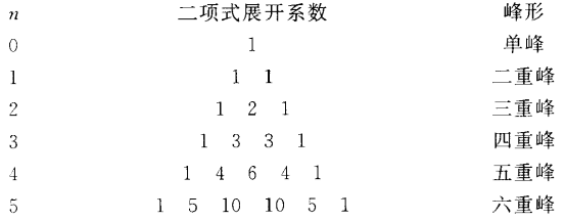
\includegraphics[width=0.7\linewidth]{image/chp6_split}
	\caption{裂分峰的强度比}
	\label{fig:chp6split}
\end{figure}

\subsection{耦合常数}

\begin{definition*}{耦合常数}{}
	耦合常数$J$:谱线裂分所产生的裂距,反映两个核之间的作用力强弱,单位Hz。与两核之间相隔的化学键数目关系很大。在$J$的左上方标以两核相距的化学键数目。
\end{definition*}

\begin{itemize}
	\item $^{2}J$:同碳上的氢,无耦合。不同种磁性核时,有耦合。
	\item $^{3}J$:相邻碳上的氢。如$\ce{H_A-CH2-CH2-H_B}$,$\ce{H_A}$与$\ce{H_B}$的耦合。
	\item $^{4}J$:相隔4个化学键,耦合作用很弱。若$J\neq 0$,则称长程耦合。
\end{itemize}

\section{电化学的基本概念}
%4、熟悉一级谱图的解析。

\subsection{常见化合物的质子位移}

\section{电化学的基本概念}
%5、了解核磁共振波谱仪的基本组成及各部分功能,了解样品的制备。

\section{电化学的基本概念}
%6、简要了解碳-13谱,和氢谱相比,有什么特点?

\section{电化学的基本概念}
